\documentclass[a4paper, 10pt]{article}
\usepackage[utf8]{inputenc}
%\usepackage[brazil]{babel}
\usepackage[top=3cm,left=3cm,right=2cm,bottom=2cm]{geometry} % para as margens
\usepackage{graphicx} % para as figuras  
\usepackage{color}
\usepackage{hyperref}
\usepackage{listings}

\newcommand{\ee}{CHOReOS Enactment Engine}


\title{How to package services to be deployed \\ by the \ee}
\author{Leonardo Leite (IME - USP)}

\begin{document}

\maketitle

\section{Introduction}

The \ee\ provides a Platform as a Service (PaaS) that automates the distributed deployment of service choreographies in cloud environments. The client of our middleware must build a declarative description of the choreography to be deployed. The description is passed to the \ee\ through a REST request. Such declarative description is a low level architectural description of the choreography, that must be writing in XML format and structured according to the relations in the Figure~\ref{img:data_model}. Details about how to build this description and how to invoke the REST operations are provided in the document ``\ee\ REST API''\footnote{\url{http://ccsl.ime.usp.br/baile/files/ee\_rest\_api.pdf}}. 

\begin{figure}[th]
\centering
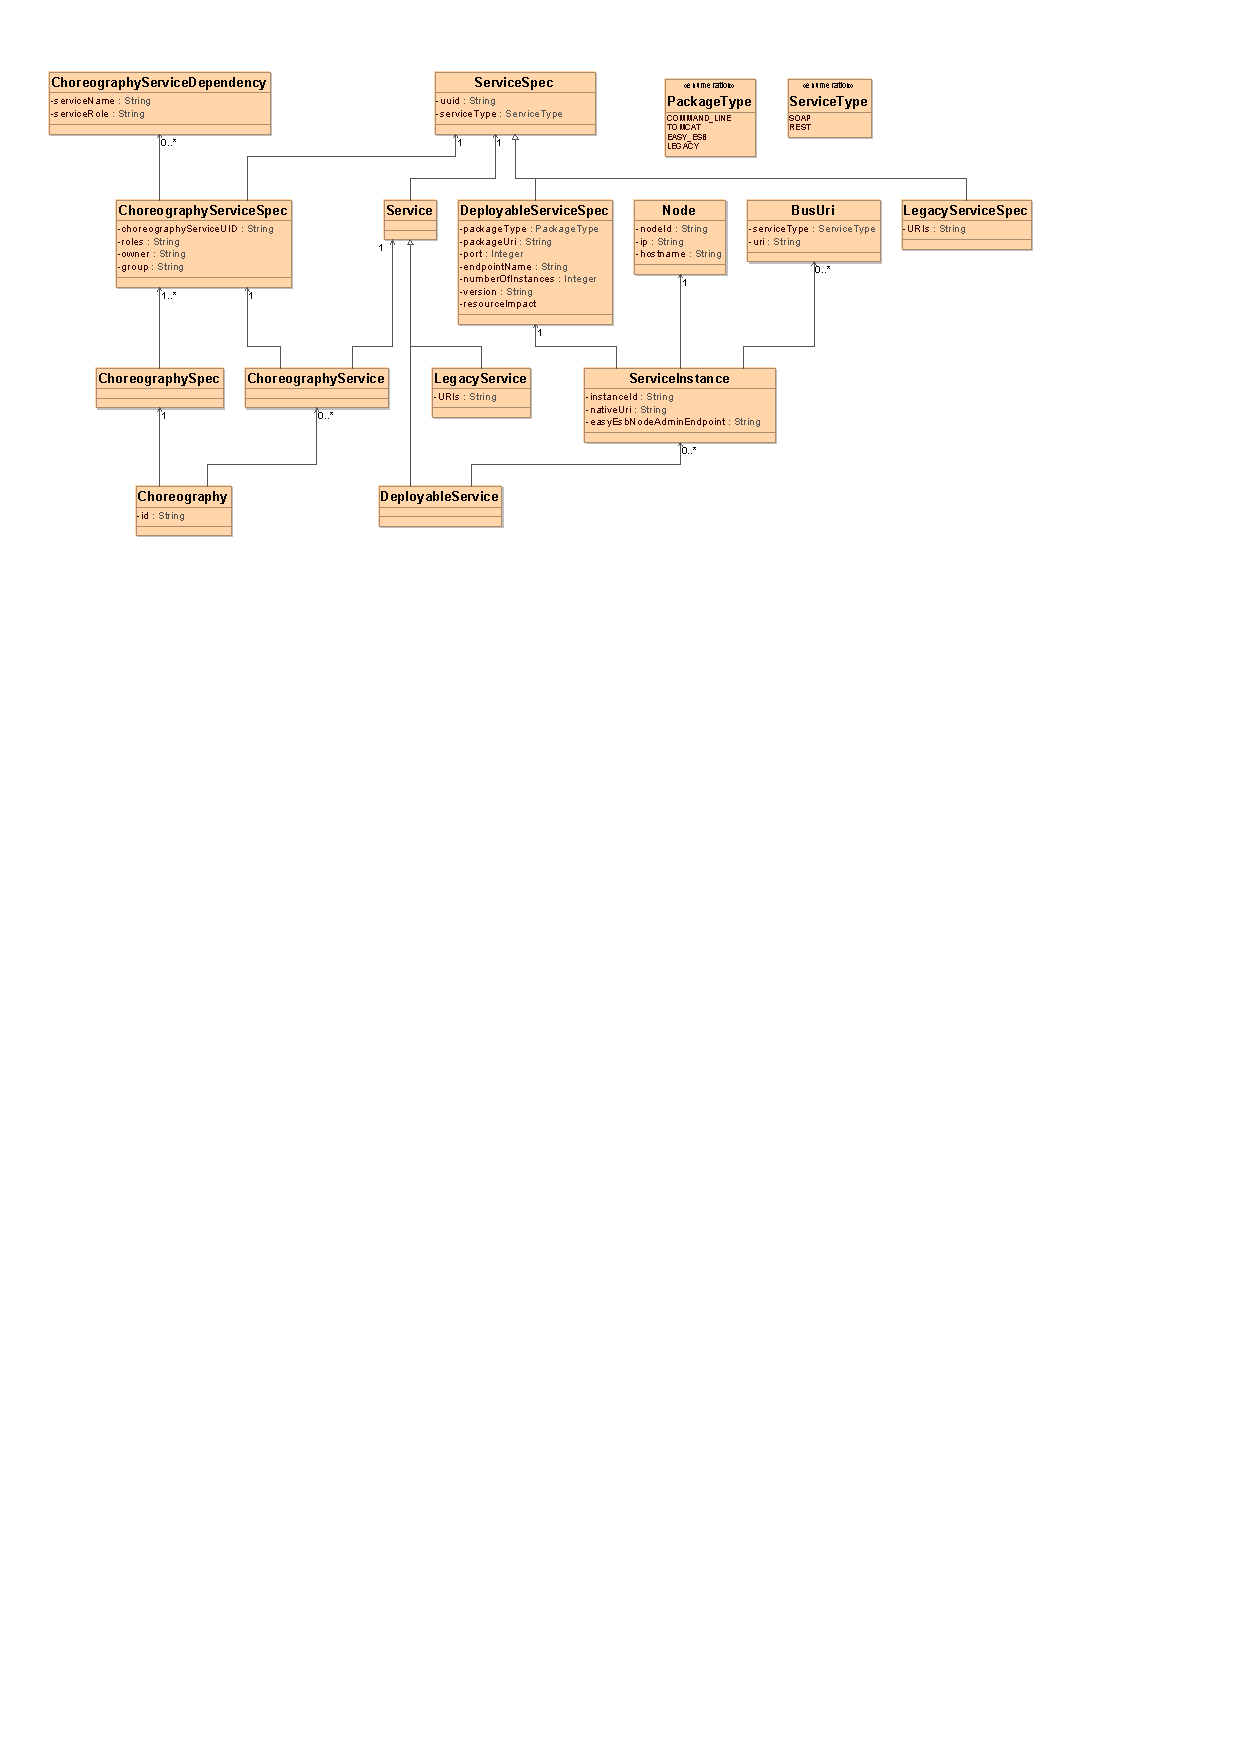
\includegraphics[scale=0.75]{img/data_model.pdf}
\caption{\ee\ REST API data model}
\label{img:data_model}
\end{figure}

Each service has its own specification, defined by the \textsf{ServiceSpec} class. Its \texttt{codeUri} attribute defines the URL from where the \ee\ retrieves the artifact that will be deployed to make the service accessible. Therefore, all the choreography artifacts need to be already Internet accessible at enactment time. This can be accomplished, for example, by hosting the artifacts on a web server.

There are two main attributes in the \textsf{ServiceSpec} class that define constrains on how a service must be coded and packaged. The \texttt{artifactType} attribute defines which kind of deployable artifact is expected by the \ee\ and, therefore, the process of deploying and running the specified service. Examples of artifact types are COMMAND\_LINE and TOMCAT. The \texttt{serviceType} attribute defines the process of invoking the specified service, which is used by the \ee\ to properly invoke the \texttt{setInvocationAddress} operation during enactment. Examples of service types are SOAP and REST types, although only SOAP services are currently supported by the \ee.

Although the amount of artifact and service types currently supported are quite limited, the \ee\ was designed with an extensible architecture that enables developers to easily provide support to new types by simply creating new implementations of already defined interfaces.

In this document we will provide details about each artifact type and service type already supported by the \ee, as well as present some service coding guidelines. 

\section{COMMAND\_LINE artifact type}

Services whose artifact type are specified as COMMAND\_LINE must be provided as JAR packages. The JAR must contain all the dependencies and resources within it. When using this artifact type, it is mandatory to fill the attributes \texttt{port} and \texttt{endpointName} on \textsf{ServiceSpec}.

It must be possible to run the JAR by typing the command \texttt{java -jar <file\_name>}, where \texttt{<file\_name>} must be replaced with the name of the JAR file. Every JAR file contains a file called \texttt{MANIFEST.MF} within the \texttt{META-INF} folder, which is in the root of JAR file. A runnable JAR contains the following entry in its \texttt{MANIFEST} file: ``\texttt{Main-Class: <class>}'', where \texttt{<class>} must be replaces by the full qualified name of the class containing the main method, as for example \texttt{org.ow2.choreos.AirlineStarter}.

The Listing~\ref{lst:jar_main_class} provides an example of main class within a JAR file. The \textsf{Airline} interface is the business interface, and the \textsf{AirlineService} is the implementing class that uses the JAX-WS framework to expose SOAP services. In this example, the used TCP port and the endpoint name are defined in the SERVICE\_ADDRESS assignment (line 7). The used port is the 1234, and the endpoint name is ``airline''. \emph{Attention!} The use of ``0.0.0.0'' instead of ``localhost'' is necessary to make the service accessible from outside the machine where it is running. 


\lstset{
language=Java,
numbers=left
}

{\footnotesize
\begin{lstlisting}[caption=Example of a class with the main method within a JAR file, label=lst:jar_main_class]
package org.ow2.choreos;

import javax.xml.ws.Endpoint;

public class AirlineStarter {

  public static final String SERVICE_ADDRESS = ``http://0.0.0.0:1234/airline'';
  private static Endpoint endpoint;
	
  public static void start() {
    Airline service = new AirlineService();
    endpoint = Endpoint.create(service);
    endpoint.publish(SERVICE_ADDRESS);
  }

  public static void main(String[] args) {	
    start();
  }
}
\end{lstlisting}
}

Runnable JARs can be easily generated by the export menu in Eclipse or by Maven. To generate a runnable JAR using Maven 3, add the excerpt in the Listing~\ref{lst:pom_runnable_jar} in your \texttt{pom.xml} file, properly replacing the content of the \texttt{mainClass} element. In this way, when generating the JAR file, Maven will be in charge of properly generating the \texttt{MANIFEST} file.

\lstset{
language=XML
}

{\footnotesize
\begin{lstlisting}[caption=Excerpt of pom file to generate a runnable JAR using Maven 3, label=lst:pom_runnable_jar]
<build>
  <finalName>airline-service</finalName> 
  <!-- <finalName>travel-agency-service</finalName> -->
  <plugins>
    <plugin>
      <groupId>org.apache.maven.plugins</groupId>
      <artifactId>maven-shade-plugin</artifactId>
      <version>2.0</version>
      <executions>
        <execution>
          <phase>package</phase>
          <goals>
            <goal>shade</goal>
          </goals>
          <configuration>
            <shadedArtifactId>airline-service</shadedArtifactId>
            <shadeSourcesContent>true</shadeSourcesContent>
            <transformers>
                <transformer 
implementation=``org.apache.maven.plugins.shade.resource.ManifestResourceTransformer''>
                <mainClass>org.ow2.choreos.AirlineStarter</mainClass>
              </transformer>
            </transformers>
          </configuration>
        </execution>
      </executions>
    </plugin>
  </plugins>
</build>
\end{lstlisting}
}

An important issue about using JAR packages is that the \ee\ is not able to prevent TCP port conflicts. Therefore, try to avoid the use of the same port in multiple services. Also, be sure that the required ports are not blocked by the cloud infrastructure. However, a better way to prevent such port issues is not using JAR packages, but using WAR packages instead.

A good practice when generating JAR files is that a single JAR file must be able to run over different environments. This can be accomplished if configuration files are placed by the side of the JAR file, rather then packaged within it. Because of that, the \ee\ must also support the deployment of JAR files that are provided within another package (e.g. tar.gz), since this higher-level package can contain the JAR file and the necessary configuration files. However, this feature is not yet available.

\section{TOMCAT artifact type}

Services whose artifact type are specified as TOMCAT must be provided as WAR packages. The \ee\ will be in charge of deploying and starting a Tomcat instance, or select an already running instance, and then deploying the WAR package in the selected instance. If the service port is not specified in the service specification, the middleware assumes the port as 8080, the Tomcat default port. If the endpoint name is not specified, it is assumed as the WAR file name, without the ``war'' extension, as it is the default behavior in Tomcat.  

Dependencies (JAR libraries) must be packaged within the WAR file. However, we provide a set of libraries in our Tomcat installation that are usually used in Java projects, specially projects using the JAX-WS framework. If some of these JARs are used by your service, they are not required to be packaged within your WAR file, since they are already on the Tomcat class path. This strategy helps in decreasing the size of WAR files and, therefore, decreasing the deployment time. The provided libraries are the following:

\begin{itemize}
\item \verb! activation-1.1.jar!
\item \verb! ecj-3.7.1.jar!
\item \verb! gmbal-api-only-3.1.0-b001.jar!
\item \verb! ha-api-3.1.8.jar!
\item \verb! istack-commons-runtime-2.2.1.jar!
\item \verb! javax.annotation-3.1.1-b06.jar!
\item \verb! jaxb-api-2.2.3.jar!
\item \verb! jaxb-impl-2.2.4-1.jar!
\item \verb! jaxws-api-2.2.5.jar!
\item \verb! jaxws-rt-2.2.5.jar!
\item \verb! jsr181-api-1.0-MR1.jar!
\item \verb! management-api-3.0.0-b012.jar!
\item \verb! mimepull-1.6.jar!
\item \verb! policy-2.2.2.jar!
\item \verb! resolver-20050927.jar!
\item \verb! saaj-api-1.3.3.jar!
\item \verb! saaj-impl-1.3.10.jar!
\item \verb! stax-api-1.0-2.jar!
\item \verb! stax-api-1.0.1.jar!
\item \verb! stax-ex-1.4.jar!
\item \verb! stax2-api-3.1.1.jar!
\item \verb! streambuffer-1.2.jar!
\item \verb! tomcat-api.jar!
\item \verb! tomcat-jdbc.jar!
\item \verb! tomcat-util.jar!
\item \verb! tomcat_libs.tar.gz txw2-20090102.jar!
\item \verb! woodstox-core-asl-4.1.1.jar!
\item \verb! wstx-asl-3.2.3.jar!
\end{itemize}


If you write your web service using JAX-WS, your WAR file must also package a \texttt{sun-jaxws.xml} file, as Listing~\ref{lst:sun_jaxws_xml}. As any other WAR file, it must also contain a \texttt{web.xml} file. If your service was built with JAX-WS, your \texttt{web.xml} file must be similar to the one presented in the Listing~\ref{lst:web_xml}. Be aware that besides the usual definition of \texttt{servlet} and \texttt{servelet-mapping} elements, it is also necessary to declare the \texttt{listener} element exactly as in the example (lines 8, 9, and 10)\footnote{The instructions about the \texttt{sun-jaxws.xml} and \texttt{web.xml} files were retrieved from \url{http://www.mkyong.com/webservices/jax-ws/deploy-jax-ws-web-services-on-tomcat/}}.

{\footnotesize
\begin{lstlisting}[caption=Example of \texttt{sun-jaxws.xml} file, label=lst:sun_jaxws_xml]
<?xml version=``1.0'' encoding=``UTF-8''?>
<endpoints
  xmlns=``http://java.sun.com/xml/ns/jax-ws/ri/runtime''
  version=``2.0''>
  <endpoint
      name=``Airline''
      implementation=``org.ow2.choreos.AirlineService''
      url-pattern=``/airline''/>
</endpoints>
\end{lstlisting}
}

{\footnotesize
\begin{lstlisting}[caption=Example of \texttt{web.xml} file, label=lst:web_xml]
<?xml version=``1.0'' encoding=``UTF-8''?>
<!DOCTYPE web-app PUBLIC ``-//Sun Microsystems, 
Inc.//DTD Web Application 2.3//EN''
``http://java.sun.com/j2ee/dtds/web-app_2_3.dtd''>
 
<web-app>
    <listener>
        <listener-class>
                com.sun.xml.ws.transport.http.servlet.WSServletContextListener
        </listener-class>
    </listener>
    <servlet>
        <servlet-name>airline</servlet-name>
        <servlet-class>
        	com.sun.xml.ws.transport.http.servlet.WSServlet
        </servlet-class>
        <load-on-startup>1</load-on-startup>
    </servlet>
    <servlet-mapping>
        <servlet-name>airline</servlet-name>
        <url-pattern>/airline</url-pattern>
    </servlet-mapping>
    <session-config>
        <session-timeout>120</session-timeout>
    </session-config>
</web-app>
\end{lstlisting}
}

\section{EASY\_ESB artifact type}

The \ee\ is also responsible of the coordination delegates deployment, that are executed by the EasyESB service bus. To enable this functionality, we have created the EASY\_ESB artifact type, that is a tar.gz package containing a \texttt{config.xml} file with instructions for the bus. In the package, some resources needed for the deployment can be added. This process enables not only the deployment of coordination delegates, but actually any interaction with EasyESB.

The \texttt{config.xml} file must be built according to the schema in the Listing~\ref{lst:config_xml_schema}. \texttt{Configuration} is the root element. \texttt{Service} is an element containing a set of \texttt{Actions} made on a particular EasyESB node. These actions can be:

\begin{description}
\item [Deploy:] deploys an artifact in EasyESB (BPEL, CD, etc.). It must contain the \texttt{MainResource} element and can have additional \texttt{Resource} elements.
\item [Bind:] binds a running web service onto an EasyESB; this action receives as parameter the web service URL and the web service WSDL location. 
\item [Proxify:] binds a running web service onto an EasyESB node and re-export it using the same parameters used in the \texttt{Bind} action.
\item [Expose:] exposes an EasyESB internal service as a web service. Parameters are \texttt{ServiceNamespace} and \texttt{ServiceName}, that correspond to the \texttt{QName} of the service defined in the WSDL (usually it is the WSDL target namespace plus the name attribute of the service element).
\end{description}

{\footnotesize
\begin{lstlisting}[caption=\texttt{config.xml} schema, label=lst:config_xml_schema]
<?xml version="1.0" encoding="UTF-8"?>
<schema targetNamespace="http://ebmwebsourcing.com/cli/schema"
 elementFormDefault="qualified" xmlns="http://www.w3.org/2001/XMLSchema"
 xmlns:tns="http://ebmwebsourcing.com/cli/schema">

  <element name="Configuration" type="tns:ConfigurationType" />

  <complexType name="ConfigurationType">
    <sequence>
      <element maxOccurs="unbounded" name="Service"
        type="tns:ServiceConfigurationType" />
    </sequence>
  </complexType>

  <complexType name="ServiceConfigurationType">
    <sequence>
      <element maxOccurs="unbounded" name="Action" type="tns:ActionType" />
    </sequence>
    <attribute name="url" type="string" />
  </complexType>

  <complexType name="ActionType">
    <choice>
      <element name="Deploy" type="tns:DeployType" />
      <element name="Bind" type="tns:BindType" />
      <element name="Expose" type="tns:ExposeType" />
      <element name="Proxify" type="tns:ProxifyType" />
      <element name="AddNeighbourNode" type="tns:AddNeighbourNodeType" />
    </choice>
  </complexType>

  <complexType name="AddNeighbourNodeType">
    <sequence>
      <element name="NeighbourAdminAddress" type="string" />
    </sequence>
  </complexType>

  <complexType name="DeployType">
    <sequence>
      <element name="MainResource" type="string" />
      <element maxOccurs="unbounded" name="Resource" type="string" />
    </sequence>
  </complexType>

  <complexType name="BindType">
    <sequence>
      <element name="Url" type="string" />
      <element name="Wsdl" type="string" />
    </sequence>
  </complexType>

  <complexType name="ExposeType">
    <sequence>
      <element name="ServiceNamespace" type="string" />
      <element name="ServiceName" type="string" />
      <element name="EndpointName" type="string" />
    </sequence>
  </complexType>

  <complexType name="ProxifyType">
    <sequence>
      <element name="Url" type="string" />
      <element name="Wsdl" type="string" />
    </sequence>
  </complexType>

</schema>
\end{lstlisting}
}

The Listing~\ref{lst:config_xml} shows an example of \texttt{config.xml} file that makes the deployment of a coordination delegate in a scenario where the correspondent business service is already running and available\footnote{Indeed, the main scenario envisioned by CHOReOS is that there are already a lot of the services running ``on the wild'', and choreographies are made just to compose these already-running services, situation in which only coordels are actually deployed.}. The \texttt{weatherforecastservice.lts} and \texttt{cdweatherforecastservice.wsdl} files, referenced in lines 8 and 9, are provided within the tar.gz package. The use of the ``../../'' in these lines is mandatory. The url \texttt{http://192.168.56.101:8192/weatherforecastservice} provided in line 15, as well as the correspondent WSDL indicated in line 15, are references to a service already running and accessible. The \texttt{ServiceNamespace} (line 20) is the \texttt{targetNamespace} defined in the service WSDL. The value of the \texttt{ServiceName} element (line 21) must correspond to the value of the \texttt{name} attribute of the \texttt{service} element in the service WSDL. The value of the \texttt{EndpointName} element (line 22) must correspond to the \texttt{name} of the \texttt{portType} element in the coordination delegate WSDL. The lts file pointed by the \texttt{config.xml} is provided in the Listing~\ref{lst:weather_lts}, and the value of its \texttt{endpoint} attribute must correspond to the \texttt{name} of the \texttt{portType} element in the already-running service WSDL.

{\footnotesize
\begin{lstlisting}[caption=Example of \texttt{config.xml} that deploys a coordination delegate, label=lst:config_xml]
<?xml version=``1.0'' enc\begin{lstlisting}oding=``UTF-8''?>
<Configuration xmlns=``http://ebmwebsourcing.com/cli/schema'' 
               xmlns:xsi=``http://www.w3.org/2001/XMLSchema-instance''
               xsi:schemaLocation=``http://ebmwebsourcing.com/cli/schema conf-schema.xsd''>
  <Service url="http://localhost:8180/services/adminExternalEndpoint">
    <Action>
      <Deploy>
        <MainResource>../../weatherforecastservice.lts</MainResource>
        <Resource>../../cdweatherforecastservice.wsdl</Resource>
      </Deploy>
    </Action>
    <Action>
      <Bind>
        <Url>http://192.168.56.101:8192/weatherforecastservice</Url>
        <Wsdl>http://192.168.56.101:8192/weatherforecastservice?wsdl</Wsdl>
      </Bind>
    </Action>
    <Action>
      <Expose>
        <ServiceNamespace>http://services.choreos.org/</ServiceNamespace>
        <ServiceName>WeatherForecastServiceService</ServiceName>
        <EndpointName>CDWeatherForecastServicePort</EndpointName>
      </Expose>
    </Action>
  </Service>
</Configuration>
\end{lstlisting}
}

{\footnotesize
\begin{lstlisting}[caption=LTS file of a simple coordination delegate that acts as a proxy, label=lst:weather_lts] 
endpoint=WeatherForecastServicePort
\end{lstlisting}
}

\section{Choreographing services that are already running}

A service choreography can be composed of services that are running before the choreography enactment. Although a service like this do not need to be deployed by the middleware, it must be declared on the choreography specification as a LEGACY 	service in the \texttt{artifactType} attribute. The \texttt{codeUri} attribute must contain the URI to invoke the service, which will be used by the middleware to invoke the \texttt{setInvocationAddress} operation of other services. 

\section{SOAP service type}

The only service type currently supported by the \ee\ is the SOAP service type. The \texttt{setInvocationAddress} convention to this service type is that each service port type must provide an operation named ``\texttt{setInvocationAddress}'' that receives two strings. This is formally expressed with the WSDL elements presented in the Listing~\ref{lst:set_invocation_address_wsdl}. 

{\footnotesize
\begin{lstlisting}[caption=Parts of the service WSDL that define the \texttt{setInvocationAddress} operation, label=lst:set_invocation_address_wsdl] 
<xs:schema version=``1.0'' targetNamespace=``http://services.choreos.org/''>
  ...
  <xs:complexType name=``setInvocationAddress''>
    <xs:sequence>
      <xs:element name=``arg0'' type=``xs:string'' minOccurs=``0''/>
      <xs:element name=``arg1'' type=``xs:string'' minOccurs=``0''/>
    </xs:sequence>
  </xs:complexType>
  <xs:complexType name=``setInvocationAddressResponse''>
    <xs:sequence/>
  </xs:complexType>
  ...
</xs:schema>

<message name=``setInvocationAddress''>
  <part name=``parameters'' element=``tns:setInvocationAddress''/>
</message>
<message name=``setInvocationAddressResponse''>
  <part name=``parameters'' element=``tns:setInvocationAddressResponse''/>
</message>

<portType ... >
...
  <operation name=``setInvocationAddress''>
    <input message=``tns:setInvocationAddress''/>
    <output message=``tns:setInvocationAddressResponse''/>
  </operation>
</portType>
\end{lstlisting}
}

If you are using the JAX-WS framework, you can easily create a compatible \texttt{setInvocationAddress} operation by using the code provided in the Listing~\ref{lst:set_invocation_address_jax_ws}.

\lstset{
language=Java
}

{\footnotesize
\begin{lstlisting}[caption=Implementing \texttt{setInvocationAddress} with JAX-WS, label=lst:set_invocation_address_jax_ws] 
@WebService
public class SomeWebServiceClass {

    ...
    
    @WebMethod
    public void setInvocationAddress(String role, String endpoint) {
		...
    }
}
\end{lstlisting}
}

\section{Coding guidelines}

Here are just some few important reminders:

\begin{itemize}

\item Do not forget to unblock the TCP ports used by your services. Often, this may be accomplished by the usage of management tools of your cloud environment.

\item WAR packages are preferable to JAR packages. WAR packages avoid port conflict issues, and it is easier to manage the life-cycle of services distributed in WAR packages thanks to the management utilities of Tomcat. Life-cycle management matters, for example, when debugging if a service is actually running or not. Handling the life-cycle of JAR packaged services requires directly handling Unix processes.

\item Never use absolute paths to retrieve resources, since the service will not run in the same machine where it was compiled. A good way to access resources is using the \texttt{getResourceAsStream} method of the current class loader\footnote{\url{http://docs.oracle.com/javase/6/docs/api/java/lang/ClassLoader.html\#getResourceAsStream(java.lang.String)}}.

\item When starting a JAR packaged service, do not use the ``localhost'' address to create the endpoint, since the service will be not remotely accessible. Instead, use the address ``0.0.0.0'' that will make your service listen in every possible address in the machine, including the localhost. This practice makes the service accessible from other machines.

\item Do not use \texttt{System.out.println}, use a log tool instead. Since the services are deployed in an automated way, it must be impossible to retrieve the console output, which will make debugging harder. Using a logger, as Log4j for example, makes the service to record its messages in a file, which helps developers and operators in debugging.

\item Do not forget to validate the WSDL files of your web services, specially if there is some manual edition applied on them.


\end{itemize}


\end{document}
